\documentclass[10pt]{article}
\usepackage[polish]{babel}
\usepackage[utf8]{inputenc}
\usepackage[T1]{fontenc}
\usepackage{amsmath}
\usepackage{amsfonts}
\usepackage{amssymb}
\usepackage[version=4]{mhchem}
\usepackage{stmaryrd}
\usepackage{graphicx}
\usepackage[export]{adjustbox}
\graphicspath{ {./images/} }

\title{LIGA MATEMATYCZNA im. Zdzisława Matuskiego \\
 PAŹDZIERNIK 2018 \\
 GIMNAZJUM }

\author{}
\date{}


\begin{document}
\maketitle
(klasa VII i VIII szkoły podstawowej, klasa III gimnazjum)

\section*{ZADANIE 1.}
Wewnątrz kwadratu \(A B C D\) leży punkt \(P\). Odległość tego punktu od wierzchołków \(A, B, C\) jest równa odpowiednio 2, 7, 9. Oblicz odległość punktu \(P\) od wierzchołka \(D\).

\section*{ZADANIE 2.}
Na ile sposobów można przedstawić liczbę 3 jako sumę sześcianów pięciu liczb całkowitych? Przedstawień różniących się jedynie kolejnością składników nie uznajemy za różne.

\section*{ZADANIE 3.}
W klasie VII, liczącej 24 uczniów, średnia liczba punktów uzyskanych na klasówce wyniosła 75 na 100 możliwych do zdobycia. Maksymalną liczbę 100 punktów otrzymało 4 uczniów. Wyznacz średnią liczbę punktów zdobytych przez pozostałych 20 uczniów.

\section*{ZADANIE 4.}
Znajdź wszystkie takie liczby trzycyfrowe, że po skreśleniu cyfry setek otrzymamy liczbę dwukrotnie mniejszą niż po skreśleniu cyfry jedności.

\section*{ZADANIE 5.}
Dany jest kwadrat \(A B C D\). Oblicz miarę kąta \(\alpha\) (patrz rysunek).\\
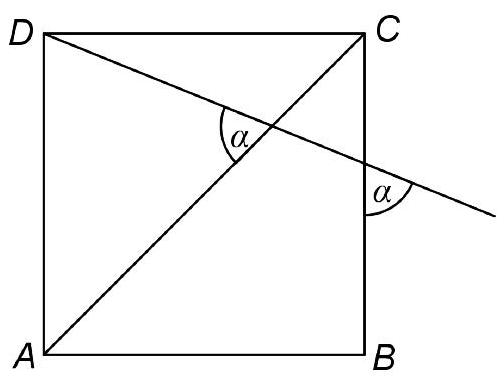
\includegraphics[max width=\textwidth, center]{2024_11_21_d79c811e6abe9c0f3ebfg-1}


\end{document}